\subsection{Control Center (CC) Module} Control Center plays an important role in this thesis. It is the eye that visualizes the internal status of the modules. It was first built for the purpose of visually render the skeletal points of the human body that is being tracked by NiTE. Later, it became one place to interact with the whole system. 

CC is developed in Javascript with the help of WebGL and jQuery. The cloud computing is day by day pushing computer applications to the Internet, which allows softwares to be operated using internet-enabled devices. Due to this reason browser based cross-compatible applications are getting popular and that leads to the huge involvement of development in Javascript. Therefore, we chose a cross-compatible platform that work out of the box than implementing the same in C++ using OpenGL.

\begin{figure}
	[h] \centering 
	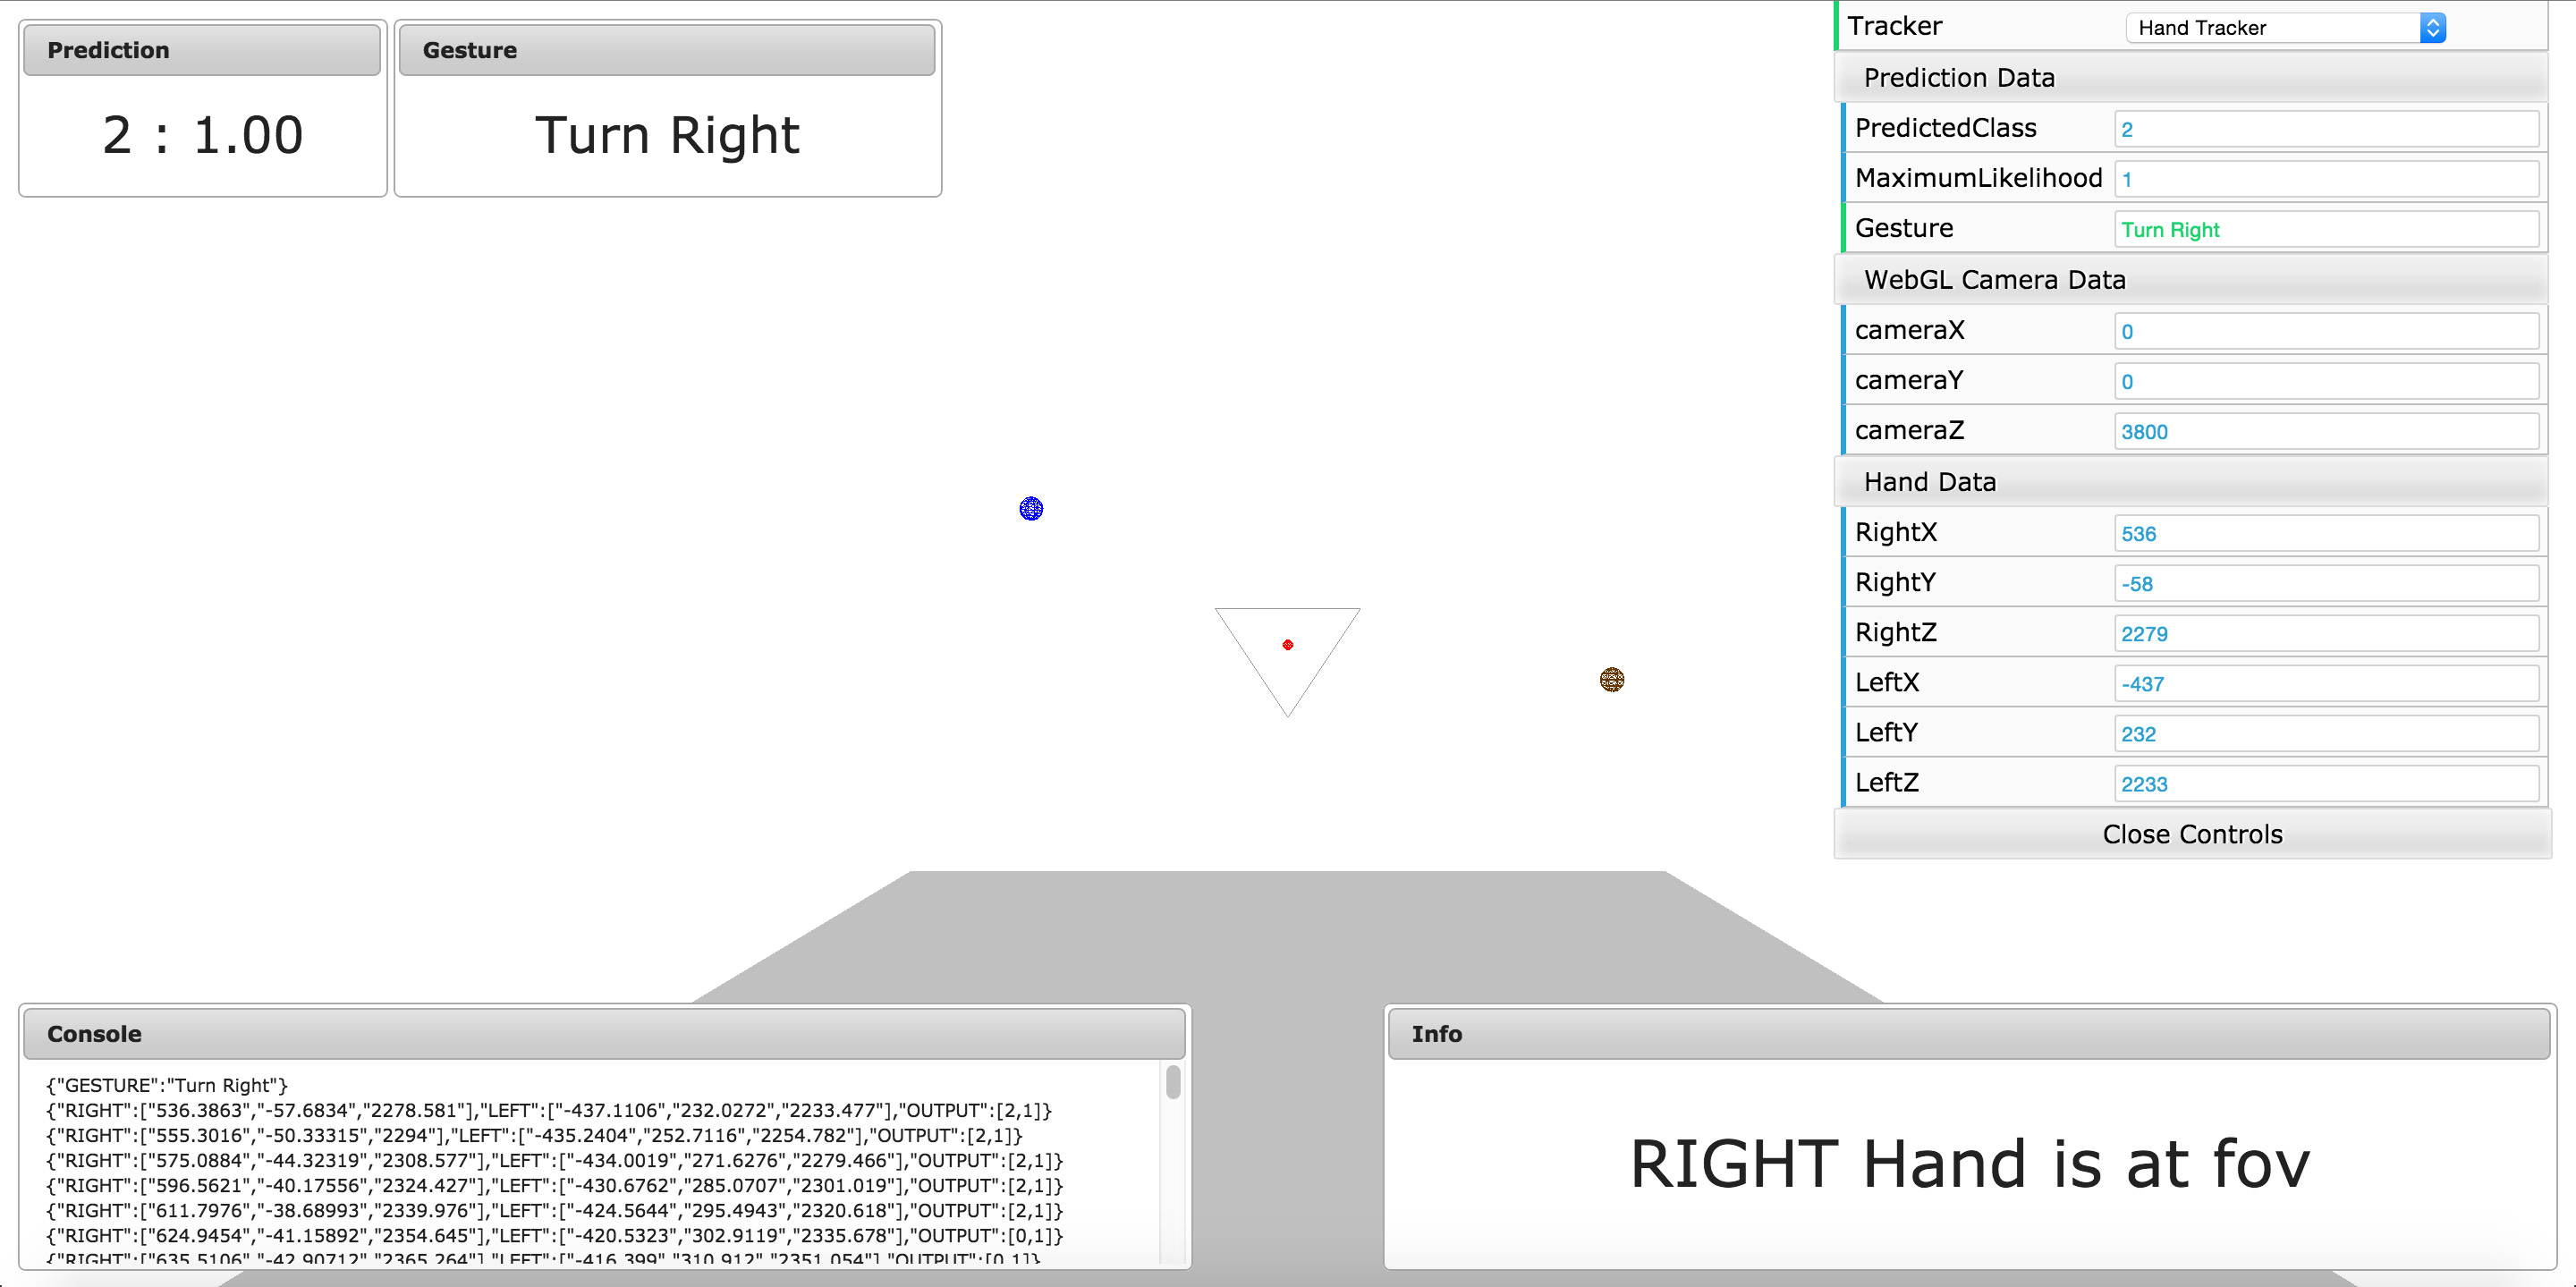
\includegraphics[width=120mm]{/content/cc-hand.jpg} \caption{Control Center displays received data of hand positions and prediction results} \label{fg:cc:hand} 
\end{figure}

\paragraph*{Javascript} It is a dynamic programming language whose implementations allow client-side scripts to interact with the user, control the browser, communicate asynchronously, and alter the document content that is displayed. However, It is also used in server-side network programming with runtime environments such as Node.js, game development and the creation of desktop and mobile applications.

\paragraph*{ThreeJS} It is a lightweight 3D library with a very low level of complexity, written purely in Javascript that can render 3D objects in various renderer such as canvas, svg, CSS3D and WebGL. In this thesis, we have chosen WebGL renderer to implement the Control Center since it is faster than others in rendering tracked skeletal points at 30 frames per second.

\paragraph*{WebSocket Client} CC receives the data from Brain modules via WebSocket. The client uses the native Javascript WebSocket implementation that is supported by many latest browsers. It connects to the WebSocket server that is listening on the port 5008. When the client receives the data, it updates the data buffer asynchronously.

\paragraph*{Architecture} Control Center is implemented in MV* (Model View) design pattern that is quite popular among Javascript developers. Since the requirement of this module needs many libraries, a dependency injection library called RequireJS is used to load all the libraries when the application is opened in the browser.  

\paragraph*{Libraries} Along with ThreeJS, libraries such as jQuery, underscore, TrackBallControl and datGUI are used in this module. jQuery is most common library for Document Object Model (DOM) manipulation in the browser. Operations on arrays and objects are made easier with the help of underscore. TrackBallControl allows to do manipulations such as rotate, revolve and transform the objects which rendered in WebGL. datGUI is a lightweight simple library to create GUI elements to build a dashboard in few lines of code.

\begin{figure}
	[h] \centering 
	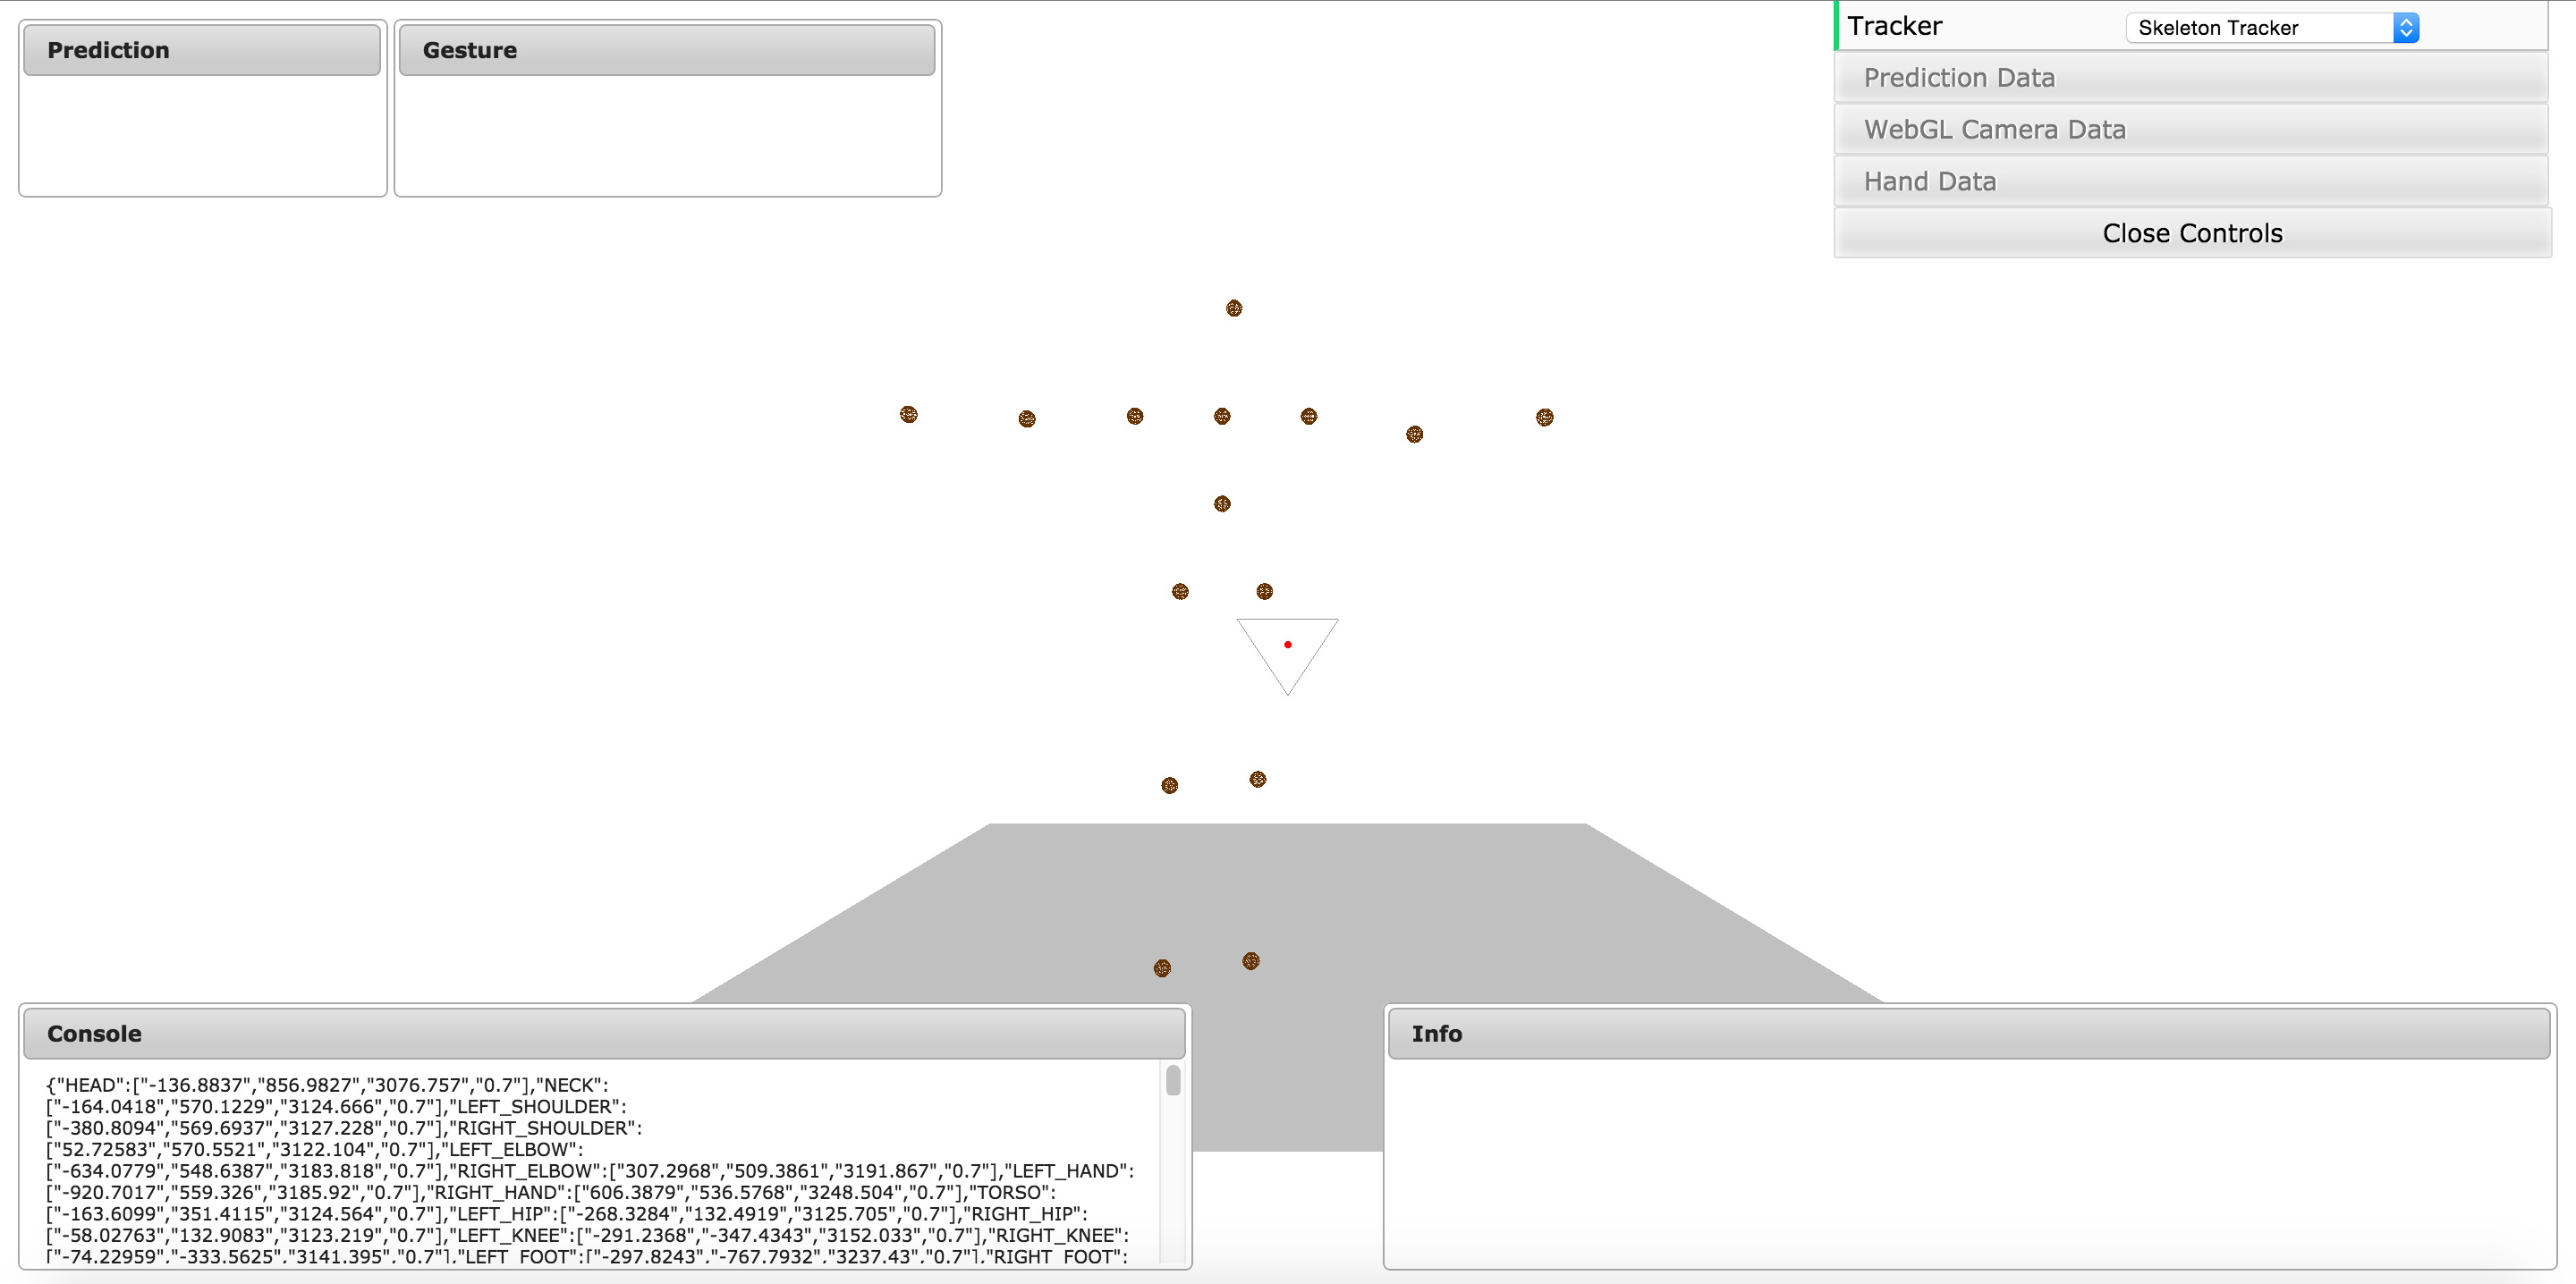
\includegraphics[width=145mm]{figures/content/cc-skeleton.jpg} 
	\caption{Control Center renders real time positions of 15 human skeleton joints.} 
	\label{fg:cc:skeleton} 
\end{figure}

\paragraph*{Model and View} To avoid complexity this Javascript application does not have any sophisticated model. It simply uses an array named skeletonBuffer that holds the JSON data received via WebSocket. All these actions are carried out in the store of the application. View does large part of the work for CC. At first it initializes the DOM and add GUI elements to it. Then ThreeJS scene is created with WebGL renderer and adds a perspective camera, a plane geometry as a base and a triangle to show origin of the sensor. By default CC is in hand tracking mode and it creates two spheres to visualize the position of left and right hand. In skeleton tracking mode it creates 15 spheres two show all the skeletal points that are being tracked by NiTE. Control Center offers us to replay the positions of joints by storing them to a file and selecting Hand Tracker From Data option in the GUI. View automatically iterates through all the objects in the array and renders them at 60 fps. 

\paragraph*{User Interface (UI) } Figure \ref{fg:cc:hand} the dashboard of the Control Center. Console box is an UI element that shows all the incoming data via WebSocket. It allows us to scroll through the data, if there is a necessity to cross check the data. Right bottom shows Info box which is created for the purpose of showing all intercommunication messages among all the modules. For example, "RIGHT Hand is at FOV" is an info message triggered by NiTE to inform that hand is closer to the field of view (FOV) and it may lose the hand. Left top corner displays two UI elements which are meant to show the prediction result for every input sample and recognized gesture  that is triggered only after gesticulating it for more than one second. Furthermore, top right corner of the dashboard reveals more internal variables such as WebGL camera positions and real time hand in 3 dimensional Cartesian coordinates. CC can not only render hand joints, but also complete human skeleton with 15 skeletal point which are being tracked as shown in the figure \ref{fg:cc:skeleton}. It also allows us to save tracking data to a json file and replay them by choosing appropriate mode from the drop down list on the top right corner.



